% Reporte Académico Oficial - Proyecto: Algoritmos de Ordenamiento Paralelos
% Curso: Estructuras de Datos y Algoritmos II (EDA II)
% Facultad de Ingeniería, UNAM - Semestre 2026-1 / 2027-1
% Grupo 11 - Profesor: M.I. José Rodrigo Moreno López
\documentclass[11pt,letterpaper,oneside]{article}
\usepackage[spanish,es-nodecimaldot,es-noshorthands]{babel}
\addto\captionsspanish{\renewcommand{\tablename}{Tabla}}

\usepackage{iftex}
\ifPDFTeX
  \usepackage[utf8]{inputenc}
  \usepackage[T1]{fontenc}
  \usepackage{tgpagella}
\else
  \usepackage{fontspec}
  \IfFontExistsTF{texgyrepagella-regular.otf}{
    \setmainfont{texgyrepagella-regular.otf}[
      BoldFont=texgyrepagella-bold.otf,
      ItalicFont=texgyrepagella-italic.otf,
      BoldItalicFont=texgyrepagella-bolditalic.otf]
  }{
    \setmainfont{DejaVu Serif}
  }
\fi

\usepackage[margin=2.5cm,headheight=15pt]{geometry}
\usepackage{microtype}
\usepackage{amsmath,amssymb}
\usepackage{graphicx,pdfpages}
\usepackage{booktabs,tabularx,array}
\usepackage{enumitem}
\usepackage{caption}
\usepackage{needspace}
\usepackage{fancyhdr}
\usepackage[hidelinks,unicode]{hyperref}

\hypersetup{
  pdftitle={Proyecto: Algoritmos de Ordenamiento Paralelos},
  pdfauthor={Angel Joseph Estrada Santos, Hanniel Cardoso Jaramillo, Luis Ricardo Mondragon Zuniga},
  pdfsubject={Estructuras de Datos y Algoritmos II - UNAM FI}
}

\graphicspath{{figuras/}}
\setlength{\parindent}{1.2em}
\setlength{\parskip}{0.25em}
\setlength{\emergencystretch}{2em}
\setlist[itemize]{topsep=4pt,itemsep=3pt,leftmargin=*}
\captionsetup{font=small,labelfont=bf}
\widowpenalty=10000
\clubpenalty=10000
\displaywidowpenalty=10000
\raggedbottom

\pagestyle{fancy}
\fancyhf{}
\fancyhead[L]{\small EDA II · Proyecto Especial}
\fancyhead[R]{\small Algoritmos de Ordenamiento Paralelos}
\fancyfoot[C]{\thepage}

\DeclareRobustCommand{\archivo}[1]{\texttt{\detokenize{#1}}}
\pdfstringdefDisableCommands{\def\archivo#1{\detokenize{#1}}}

\begin{document}

% Inclusión de la carátula oficial de la Facultad de Ingeniería
\ifdefined\PortadaPDF
  \IfFileExists{\PortadaPDF}{%
    \hypersetup{pageanchor=false}
    \includepdf[pages=1,pagecommand={\thispagestyle{empty}}]{\PortadaPDF}
    \hypersetup{pageanchor=true}
  }{}
\else
  \IfFileExists{portada.pdf}{%
    \hypersetup{pageanchor=false}
    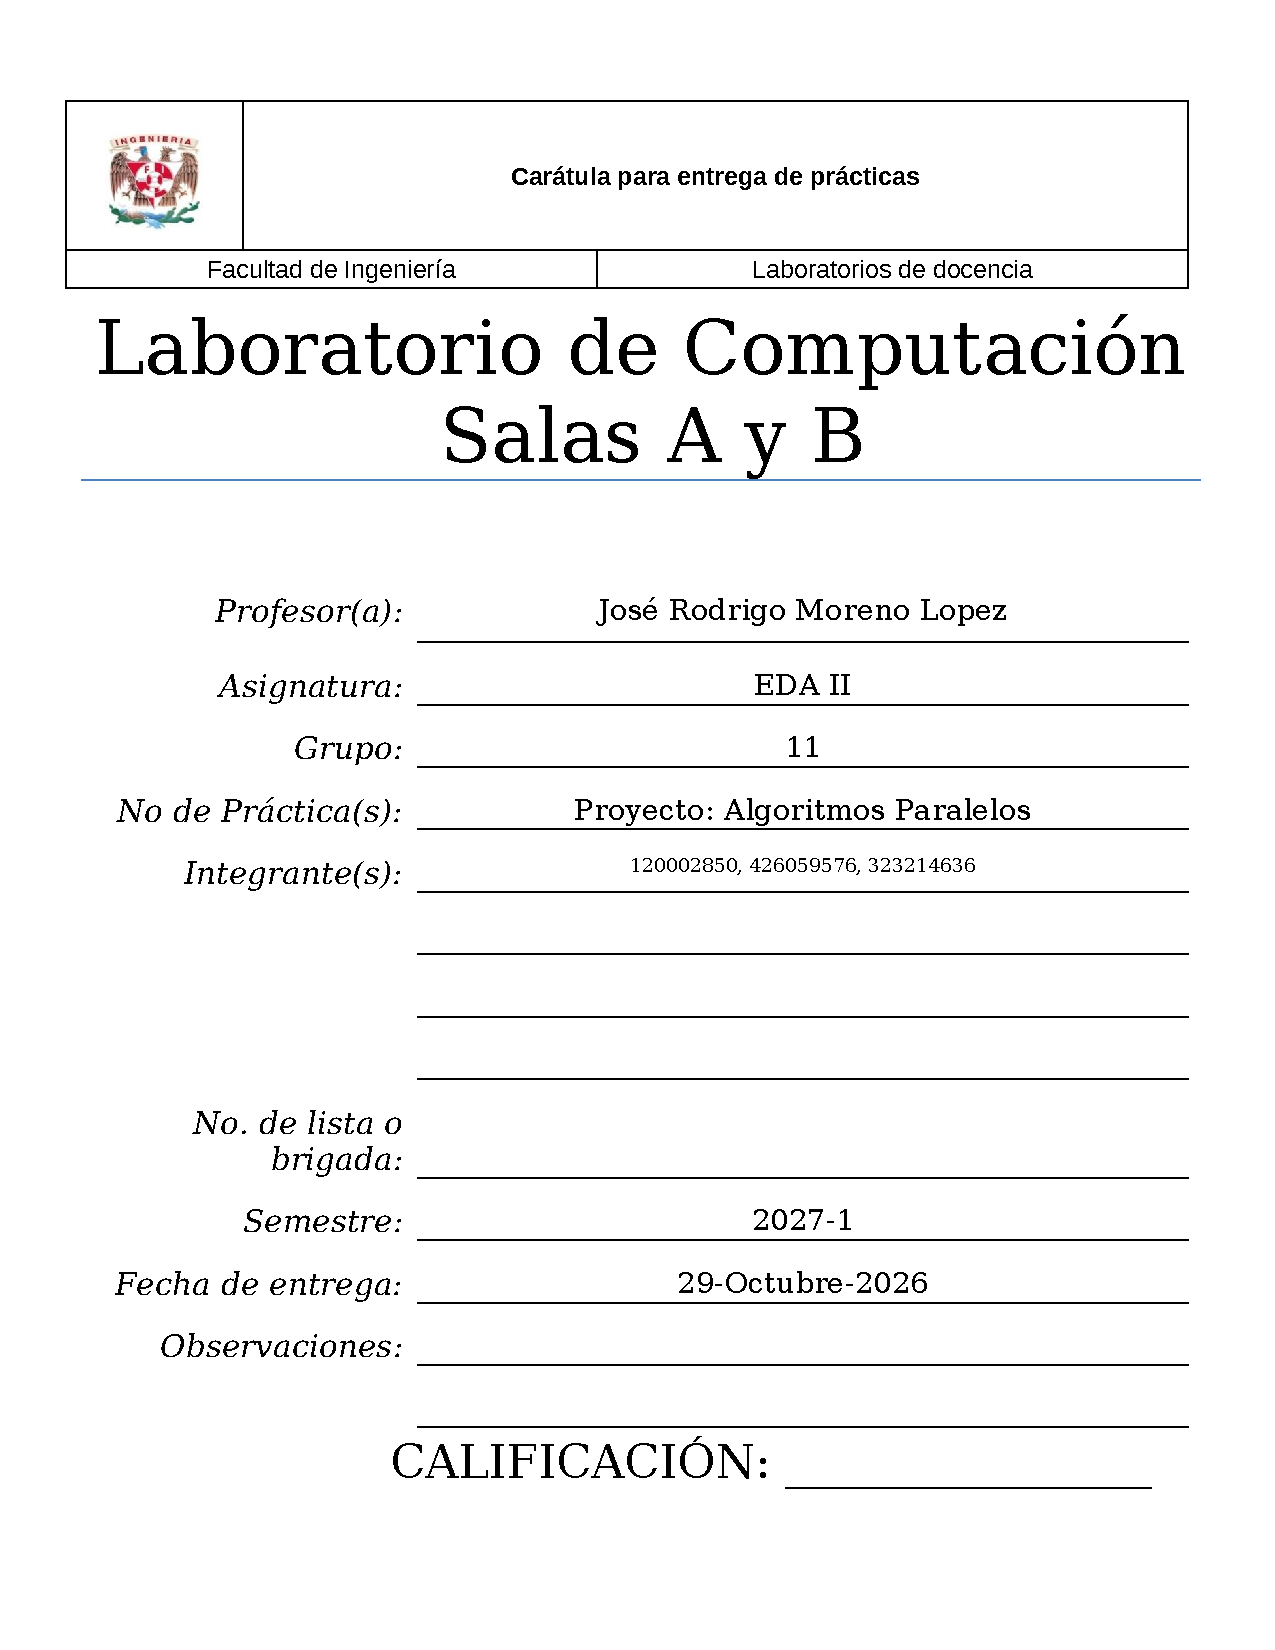
\includepdf[pages=1,pagecommand={\thispagestyle{empty}}]{portada.pdf}
    \hypersetup{pageanchor=true}
  }{}
\fi

\pagenumbering{arabic}
\hypersetup{pageanchor=true}

\begin{center}
  {\Large\bfseries Algoritmos de Ordenamiento Paralelos:}\par
  \smallskip
  {\Large\bfseries Simulación Interactiva y Análisis de Escalabilidad}\par
  \medskip
  {\large Proyecto de Simulación · EDA II · MADO}\par
  \bigskip
  \textbf{Integrantes del Equipo (PR \#27):}\par
  \smallskip
  Angel Joseph Estrada Santos · Cuenta \textbf{120002850}\par
  Hanniel Cardoso Jaramillo · Cuenta \textbf{426059576}\par
  Luis Ricardo Mondragón Zúñiga · Cuenta \textbf{323214636}\par
  \medskip
  Profesor: M.I. José Rodrigo Moreno López · Grupo 11\par
  Facultad de Ingeniería, Universidad Nacional Autónoma de México\par
  \smallskip
  \small Preparación y despliegue: 29 de octubre de 2026, America/Mexico\_City.\par
  Sitio web público: \url{https://juxdeveloper.github.io/algoritmos/}
\end{center}

\begin{abstract}
El ordenamiento paralelo constituye una de las áreas fundamentales del cómputo de alto rendimiento, donde la concurrencia permite trascender la cota secuencial inferior de comparaciones $\Omega(n \log n)$ en términos de tiempo de ejecución (lapso o \emph{span}). En este trabajo se presenta el diseño, fundamentación matemática e implementación de un laboratorio interactivo desarrollado en React y HTML5 que ilustra, paso a paso y de forma intuitiva, ocho algoritmos de ordenamiento paralelos representativos de diversos paradigmas de hardware (PRAM, redes de comparadores, mallas bidimensionales, arquitecturas de memoria compartida y memoria distribuida con paso de mensajes). Se analizan detalladamente el trabajo $T_1$, la profundidad $T_\infty$, el \emph{speedup} teórico y real, las barreras de sincronización y las restricciones de concurrencia impuestas por el GIL (\emph{Global Interpreter Lock}) en CPython. La plataforma se encuentra desplegada públicamente mediante GitHub Actions en GitHub Pages y versionada en el PR \#27 del repositorio oficial del curso.
\end{abstract}

\tableofcontents
\medskip

\section{Objetivos del Proyecto}
\begin{itemize}
  \item Desarrollar una aplicación web interactiva en React que modele fielmente la ejecución paralela síncrona y asíncrona de los principales algoritmos de ordenamiento, facilitando la comprensión intuitiva de la sincronización entre procesadores.
  \item Implementar generadores deterministas de pasos de ejecución para ocho algoritmos paralelos: \emph{Bitonic Sort}, \emph{Odd-Even Transposition Sort}, \emph{Parallel QuickSort}, \emph{Parallel MergeSort}, \emph{Sample Sort}, \emph{Parallel Radix Sort}, \emph{Shearsort} y \emph{Parallel Bucket Sort}.
  \item Integrar vistas complementarias en tiempo real: barras con asignación de núcleos, trazado de redes de comparadores de Batcher, diagramas de Gantt con barreras de sincronización y representaciones topológicas (mallas 2D, árboles Fork-Join y cubetas de dispersión).
  \item Contrastar empíricamente la aceleración teórica predicha por la Ley de Amdahl y el Teorema de Brent con las restricciones del modelo de procesos de CPython frente al uso de hilos (\emph{threading} vs. \emph{multiprocessing}).
  \item Configurar un flujo de integración continua (CI/CD) con GitHub Actions para compilar y desplegar automáticamente el simulador en GitHub Pages ante cualquier actualización en la rama \archivo{simulacion}.
\end{itemize}

\section{Fundamentos Teóricos del Cómputo Paralelo}

\subsection{El modelo PRAM y medidas de complejidad}
El modelo teórico estándar para algoritmos paralelos es la máquina de acceso aleatorio paralelo (PRAM, por sus siglas en inglés)~\cite{ja-ja}. Se compone de $p$ procesadores homogéneos sincronizados que operan sobre un espacio global de memoria. Según las políticas de lectura y escritura simultáneas, se clasifica en:
\begin{itemize}
  \item \textbf{EREW} (\emph{Exclusive Read, Exclusive Write}): Ningún par de procesadores puede acceder concurrentemente a la misma celda de memoria. Es el modelo más restrictivo pero más reproducible físicamente.
  \item \textbf{CREW} (\emph{Concurrent Read, Exclusive Write}): Múltiples procesadores pueden leer simultáneamente la misma posición, pero las escrituras son estrictamente exclusivas.
  \item \textbf{CRCW} (\emph{Concurrent Read, Concurrent Write}): Permite lecturas y escrituras simultáneas, resolviendo colisiones mediante prioridades (\emph{Priority}), valores comunes (\emph{Common}) o elecciones arbitrarias (\emph{Arbitrary}).
\end{itemize}

Para caracterizar el rendimiento de un algoritmo paralelo sobre una entrada de tamaño $n$ con $p$ procesadores, se definen:
\begin{itemize}
  \item \textbf{Trabajo} ($T_1$): Número total de operaciones elementales ejecutadas por un solo procesador (equivalente al tiempo de ejecución secuencial).
  \item \textbf{Lapso o Profundidad} ($T_\infty$): Tiempo de ejecución con un número ilimitado de procesadores, determinado por la ruta crítica de dependencias de datos.
  \item \textbf{Aceleración o Speedup} ($S_p$): Razón entre el tiempo secuencial y el tiempo paralelo con $p$ procesadores:
  \begin{equation}
    S_p = \frac{T_1}{T_p} \le p.
    \label{eq:speedup}
  \end{equation}
  \item \textbf{Eficiencia} ($E_p$): Fracción de utilización de los recursos computacionales asignados:
  \begin{equation}
    E_p = \frac{S_p}{p} = \frac{T_1}{p \cdot T_p} \le 1.
    \label{eq:eficiencia}
  \end{equation}
\end{itemize}

\subsection{Teorema de Brent y Ley de Amdahl}
El \textbf{Teorema de Brent}~\cite{brent} establece una cota constructiva fundamental para programar un cálculo paralelo con trabajo $T_1$ y profundidad $T_\infty$ sobre una máquina finita de $p$ núcleos:
\begin{equation}
  \frac{T_1}{p} \le T_p \le \frac{T_1 - T_\infty}{p} + T_\infty < \frac{T_1}{p} + T_\infty.
  \label{eq:brent}
\end{equation}
Si el número de procesadores $p$ es pequeño frente a la cantidad de trabajo ($p \ll T_1 / T_\infty$), el término $T_1/p$ domina y se obtiene aceleración lineal perfecta ($S_p \approx p$). Por el contrario, cuando $p \to \infty$, el tiempo converge asintóticamente a la ruta crítica $T_\infty$.

Por su parte, la \textbf{Ley de Amdahl}~\cite{amdahl} delimita el límite superior de aceleración en función de la fracción estrictamente secuencial ($s = 1 - f$) de un programa, donde $f \in [0, 1]$ representa la porción paralelizable:
\begin{equation}
  S(p) = \frac{1}{(1 - f) + \dfrac{f}{p}} \quad \implies \quad S_\infty = \lim_{p \to \infty} S(p) = \frac{1}{1 - f}.
  \label{eq:amdahl}
\end{equation}
Si el 20\% de un algoritmo es serial ($s = 0.20$), el \emph{speedup} máximo alcanzable en cualquier supercomputadora con infinitos núcleos es estrictamente $S_\infty = 1 / 0.20 = 5\times$. Este principio rige directamente el diseño de particionadores en QuickSort y combinadores en MergeSort.

\subsection{Redes de comparadores y el Principio Cero-Uno}
Una red de clasificación está constituida por cables horizontales que transportan datos y compuertas verticales de comparación-intercambio (\emph{compare-exchange}) que operan simultáneamente en instantes discretos~\cite{knuth3}. A diferencia de los algoritmos basados en ramas de control, una red es \textbf{independiente de los datos} (\emph{data-oblivious}): las comparaciones se ejecutan en posiciones predefinidas sin importar los valores numéricos.

El \textbf{Principio Cero-Uno de Knuth} establece que:
\begin{quote}
\emph{«Si una red de comparadores ordena correctamente todas las $2^n$ secuencias posibles formadas únicamente por ceros y unos, entonces ordenará correctamente cualquier secuencia de $n$ elementos arbitrarios ordenables.»}
\end{quote}
Este teorema simplifica formalmente la verificación de redes como Bitonic Sort y Odd-Even Transposition.

\section{Catálogo de Algoritmos Paralelos Implementados}

En la Tabla~\ref{tab:complejidades} se resumen las características de los ocho algoritmos desarrollados en la plataforma.

\begin{table}[htbp]
\centering
\small
\caption{Complejidad teórica, modelo de hardware y propiedades de los ocho algoritmos implementados en el simulador.}
\label{tab:complejidades}
\begin{tabularx}{\textwidth}{lccccX}
\toprule
\textbf{Algoritmo} & \textbf{Trabajo ($T_1$)} & \textbf{Lapso ($T_\infty$)} & \textbf{Speedup ($S_p$)} & \textbf{Estable} & \textbf{Modelo Computacional}\\
\midrule
Bitonic Sort & $O(n \log^2 n)$ & $O(\log^2 n)$ & $O(n / \log n)$ & No & Redes de Comparadores / EREW\\
Odd-Even Transp. & $O(n^2)$ & $O(n)$ & $O(n)$ & Sí & Malla Sistólica 1D / EREW\\
Parallel QuickSort & $O(n \log n)$ & $O(\log^2 n)$ & $O(p / \log p)$ & No & Fork-Join / Memoria Compartida\\
Parallel MergeSort & $O(n \log n)$ & $O(n/p + \log n)$ & $O(p)$ & Sí & Árbol de Reducción / CREW\\
Sample Sort & $O(n \log n)$ & $O(\frac{n}{p} \log \frac{n}{p})$ & $O(p)$ & No & Memoria Distribuida (MPI)\\
Parallel Radix Sort & $O(k \cdot n)$ & $O(k(\frac{n}{p} + \log p))$ & $O(p / \log p)$ & Sí & SIMD / Prefix Sums / GPU\\
Shearsort & $O(n \log n)$ & $O(\sqrt{n} \log n)$ & $O(\sqrt{n})$ & No & Malla 2D Toroidal\\
Parallel Bucket Sort & $O(n + k)$ & $O(n/p + \log p)$ & $O(p)$ & Sí$^*$ & CREW / Dispersión Concurrente\\
\bottomrule
\end{tabularx}
\end{table}

\subsection{Bitonic Sort (Red de Batcher)}
Propuesto por Ken Batcher en 1968~\cite{batcher}, construye progresivamente subsecuencias bitónicas (secuencias que primero crecen monótonamente y luego decrecen) y las transforma en secuencias monótonas mediante el operador \emph{Bitonic Merge}. Para un arreglo de tamaño $n = 2^k$, el algoritmo se organiza en $\log_2 n$ fases principales. Cada fase $k$ se subdivide en pasos con salto $j = k/2, k/4, \dots, 1$, comparando e intercambiando en paralelo los pares $(i, i \oplus j)$.

La profundidad paralela total es exactamente:
\begin{equation}
  D(n) = \sum_{k=1}^{\log_2 n} k = \frac{\log_2 n (\log_2 n + 1)}{2} = O(\log^2 n).
  \label{eq:prof_bitonic}
\end{equation}
Para $n = 16$, Bitonic Sort concluye en exactamente 10 etapas paralelas de comparación, asignando las $n/2 = 8$ compuertas por etapa entre los núcleos disponibles.

\subsection{Odd-Even Transposition Sort}
Es la paralelización del ordenamiento burbuja sobre una cadena lineal de procesadores (malla 1D sistólica). En cada etapa par, los comparadores operan sobre índices $(2i, 2i+1)$; en cada etapa impar, operan sobre $(2i+1, 2i+2)$. Como ningún índice se repite dentro de la misma fase, todas las comparaciones de una fase se ejecutan en tiempo $O(1)$ sin riesgo de colisión. El arreglo converge en a lo sumo $n$ fases paralelas.

\subsection{Parallel QuickSort con Umbral Secuencial}
En QuickSort paralelo, tras elegir el pivote y particionar el arreglo, se lanzan dos sub-tareas recursivas independientes mediante un \emph{ProcessPool} o despachador \emph{Fork-Join}. Para evitar la sobrecarga de creación de procesos y paso de mensajes en arreglos pequeños, se incorpora un umbral secuencial (\emph{threshold}):
\begin{equation}
  \text{quicksort\_paralelo}(A) = 
  \begin{cases}
    \text{quicksort\_serial}(A) & \text{si } |A| \le \text{umbral},\\
    \text{fork}(\text{menores}) \parallel \text{fork}(\text{mayores}) & \text{en otro caso.}
  \end{cases}
\end{equation}
Esta técnica es idéntica a la implementada en la Tarea 6 de la asignatura, permitiendo que los subproblemas alcancen velocidad máxima de compilación nativa en sus hojas.

\subsection{Parallel MergeSort con Árbol de Reducción}
Se divide el arreglo de $n$ elementos en $p$ bloques contiguos de tamaño $\lceil n/p \rceil$. En la \textbf{Fase 1}, los $p$ núcleos ordenan sus bloques locales en paralelo dentro de sus propias cachés L1/L2, sin requerir sincronización ni transferencias de bus. En la \textbf{Fase 2}, un árbol de fusión binaria sincronizado mediante barreras combina los bloques por parejas hasta obtener el resultado unificado.

\subsection{Sample Sort (Ordenamiento por Muestreo MPI)}
Diseñado para arquitecturas de memoria distribuida sin bus compartido~\cite{samplesort}, resuelve el problema del desbalance de carga que sufre QuickSort paralelo. El proceso se articula en cinco fases deterministas:
\begin{enumerate}
  \item \textbf{Ordenamiento local}: Cada núcleo ordena su bloque de tamaño $n/p$.
  \item \textbf{Muestreo regular}: Cada núcleo selecciona $p-1$ muestras equidistantes ($n/p^2$).
  \item \textbf{Separadores globales (\emph{Splitters})}: Un nodo coordinador recopila las $p(p-1)$ muestras, las ordena y elige $p-1$ pivotes globales que garantizan una partición equitativa del espacio de claves.
  \item \textbf{Redistribución All-to-All}: Cada proceso dispersa sus datos en cubetas y los envía por red a los procesadores destino.
  \item \textbf{Ordenamiento final}: Cada procesador ordena localmente la cubeta consolidada recibida. La concatenación de los bloques de los $p$ procesadores produce el arreglo global ordenado.
\end{enumerate}

\subsection{Parallel Radix Sort (Conteo y Escaneo de Prefijos)}
A diferencia de los ordenamientos por comparación, Radix Sort procesa las representaciones en base $b$ dígito por dígito. Para paralelizarlo sin bloqueos atómicos, se aplica el algoritmo de \textbf{Prefix Sums / Blelloch Scan}~\cite{blelloch}:
\begin{enumerate}
  \item Cada núcleo genera un histograma de frecuencias local para el dígito actual.
  \item Se realiza un escaneo de prefijos paralelo sobre la matriz de histogramas para deducir el índice global exacto de destino de cada elemento.
  \item Cada núcleo escribe sus elementos concurrentemente en el arreglo auxiliar en sus posiciones precalculadas (\emph{Parallel Scatter}), garantizando estabilidad sin contención.
\end{enumerate}

\subsection{Shearsort (Malla Bidimensional 2D)}
Shearsort organiza $n$ datos en una matriz de $r \times c$ procesadores conectados como una malla toroidal 2D~\cite{shearsort}. Ejecuta $\lceil \log_2 r \rceil + 1$ rondas compuestas por:
\begin{enumerate}
  \item \textbf{Fase de Filas}: Se ordenan todas las filas simultáneamente en orden serpenteante (filas pares hacia la derecha $\rightarrow$, filas impares hacia la izquierda $\leftarrow$).
  \item \textbf{Fase de Columnas}: Se ordenan todas las columnas simultáneamente de arriba hacia abajo ($\downarrow$).
\end{enumerate}
La inversión deliberada de sentido en filas adyacentes cancela pares fuera de orden en columnas continuas, conduciendo a convergencia en $O(\sqrt{n} \log n)$ pasos paralelos.

\subsection{Parallel Bucket Sort}
Determina concurrentemente el rango numérico $[\min, \max]$, divide el intervalo en $B = p$ cubetas uniformes y dispersa los elementos en paralelo. Posteriormente, cada procesador ordena su cubeta asignada de manera independiente, ensamblando la secuencia final sin colisiones.

\section{Arquitectura del Laboratorio Web Interactivo}

\subsection{Decisiones de diseño según la directiva \emph{frontend-design}}
Siguiendo las pautas de diseño visual avanzado, se evitó la estética de plantillas genéricas. Se adoptó una identidad técnica inspirada en sistemas operativos de tiempo real y consolas de telemetría de supercómputo:
\begin{itemize}
  \item \textbf{Paleta de sustrato}: Fondo profundo azul pizarra (\archivo{\#090d16} y \archivo{\#0f172a}) con bordes de contraste calculados (\archivo{\#1e293b} y \archivo{\#334155}).
  \item \textbf{Codificación cromática de procesadores}: Cada núcleo posee una signatura lumínica propia e invariable a lo largo de toda la interfaz:
    \begin{itemize}
      \item Core 0 (P0): Cian eléctrico (\archivo{\#38bdf8})
      \item Core 1 (P1): Orquídea violeta (\archivo{\#a855f7})
      \item Core 2 (P2): Menta esmeralda (\archivo{\#34d399})
      \item Core 3 (P3): Ámbar dorado (\archivo{\#fbbf24})
      \item P4--P7: Tonos adicionales de alta legibilidad en modo oscuro.
    \end{itemize}
  \item \textbf{Tipografía estructural}: Combinación de \emph{Plus Jakarta Sans} para títulos y navegación con \emph{JetBrains Mono} para índices de memoria, fórmulas y trazas de pseudocódigo.
\end{itemize}

\subsection{Capturas de la aplicación web en ejecución}

A continuación se documentan las distintas vistas del sistema desplegado, capturadas de forma directa sobre la versión de producción accesible en GitHub Pages.

\begin{figure}[htbp]
  \centering
  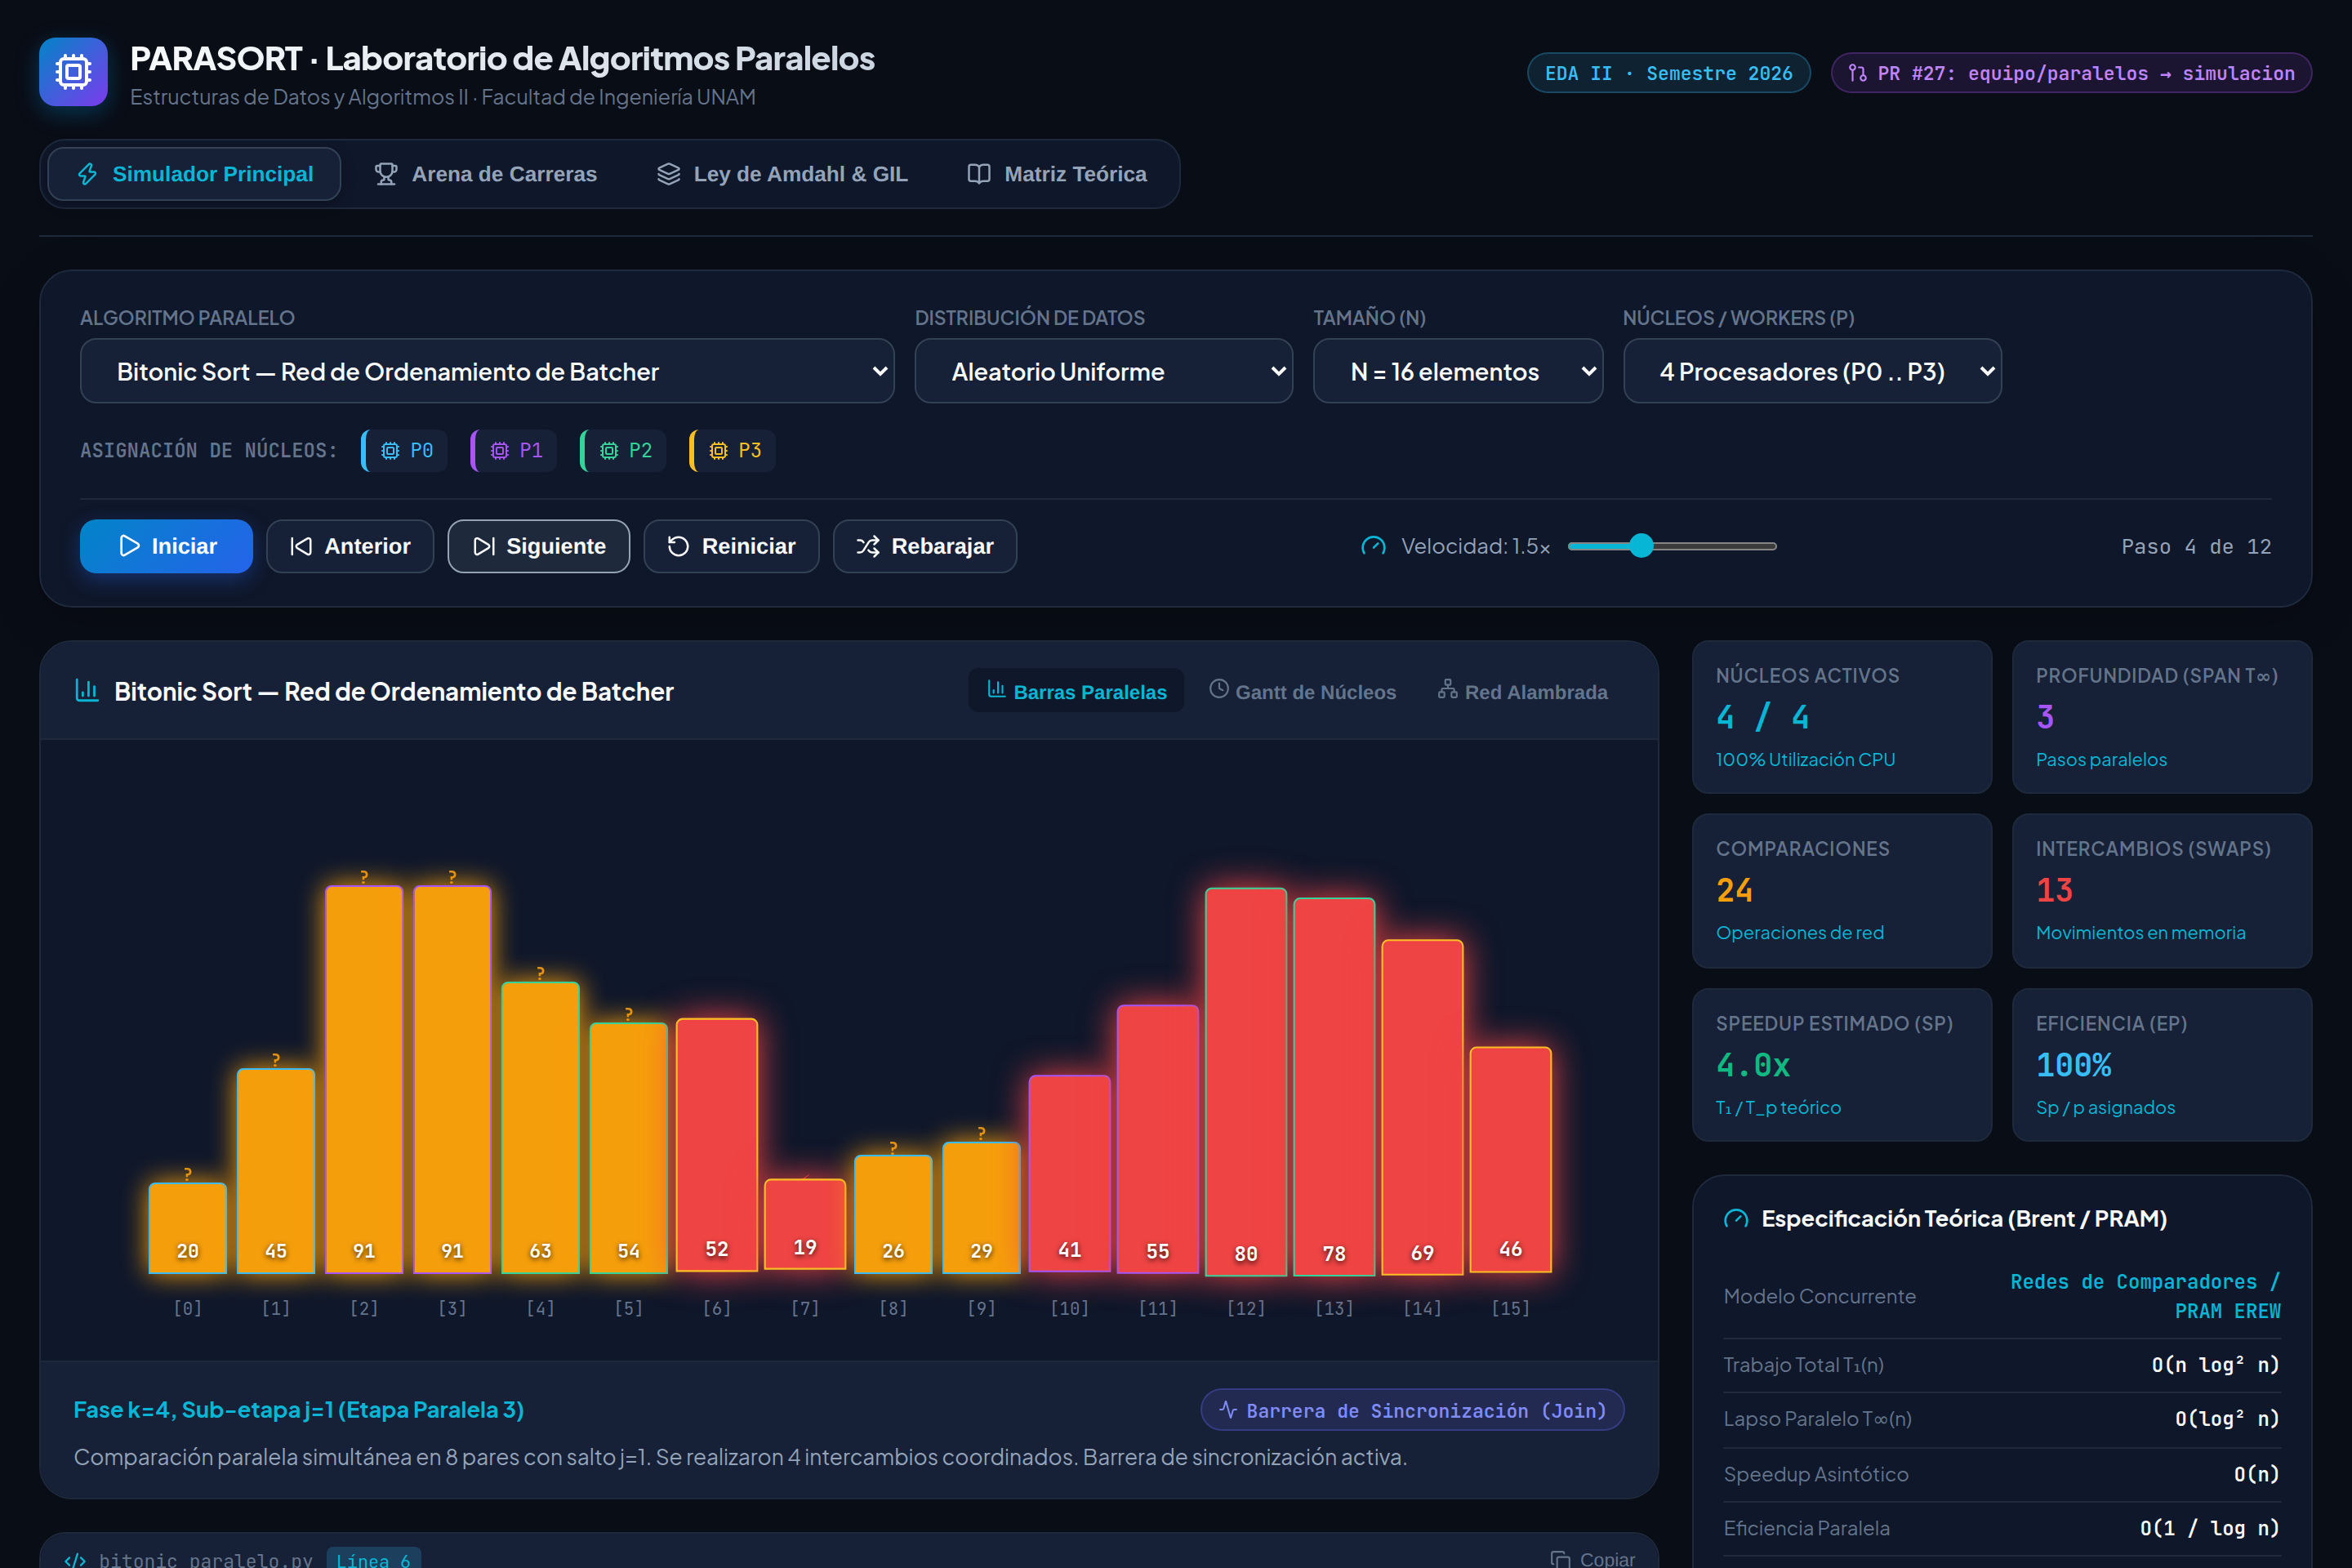
\includegraphics[width=0.95\linewidth]{simulador_principal.png}
  \caption{Simulador principal: Bitonic Sort en ejecución con 4 procesadores y $N=16$. Se observan las barras con sus etiquetas de núcleo asignado (P0..P3), el resaltado de comparaciones concurrentes en dorado, el contador de pasos paralelos y el panel de telemetría en tiempo real.}
  \label{fig:simulador}
\end{figure}

\begin{figure}[htbp]
  \centering
  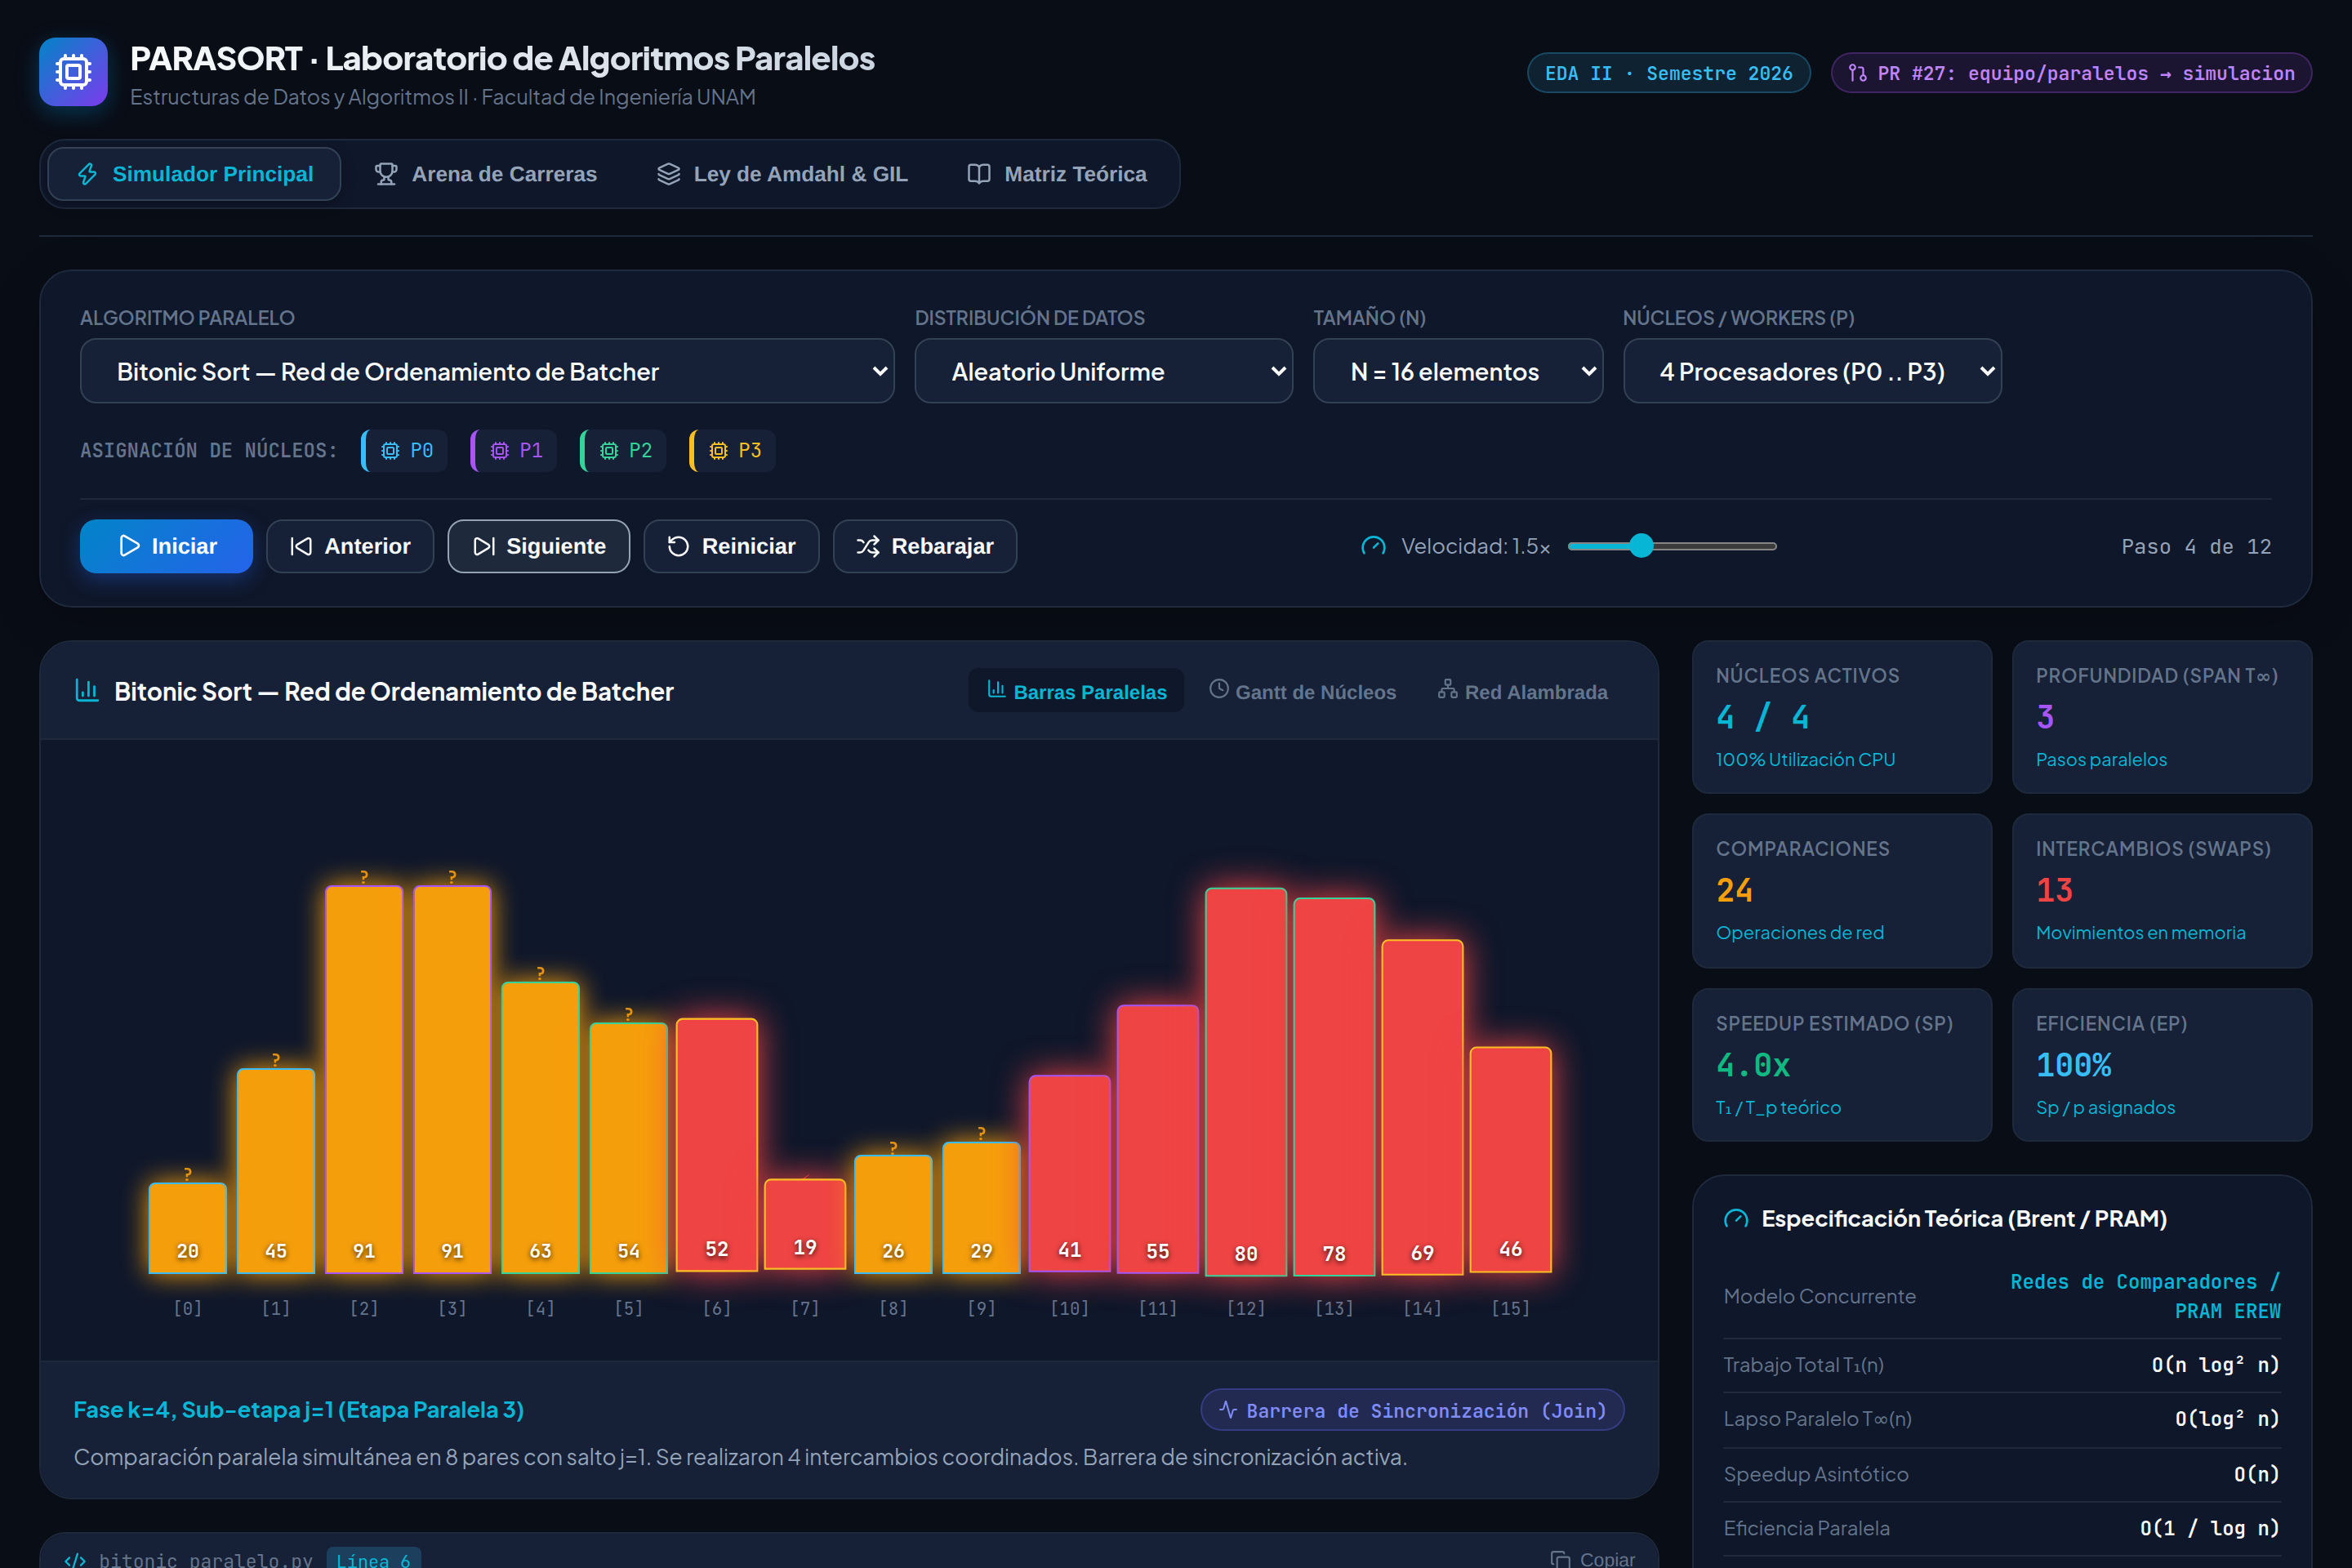
\includegraphics[width=0.95\linewidth]{red_comparadores.png}
  \caption{Visualización vectorial de la Red de Comparadores de Batcher: Alambres horizontales para cada canal de datos y compuertas lógicas verticales coloreadas por el núcleo que ejecuta la comparación-intercambio simultáneamente.}
  \label{fig:red}
\end{figure}

\begin{figure}[htbp]
  \centering
  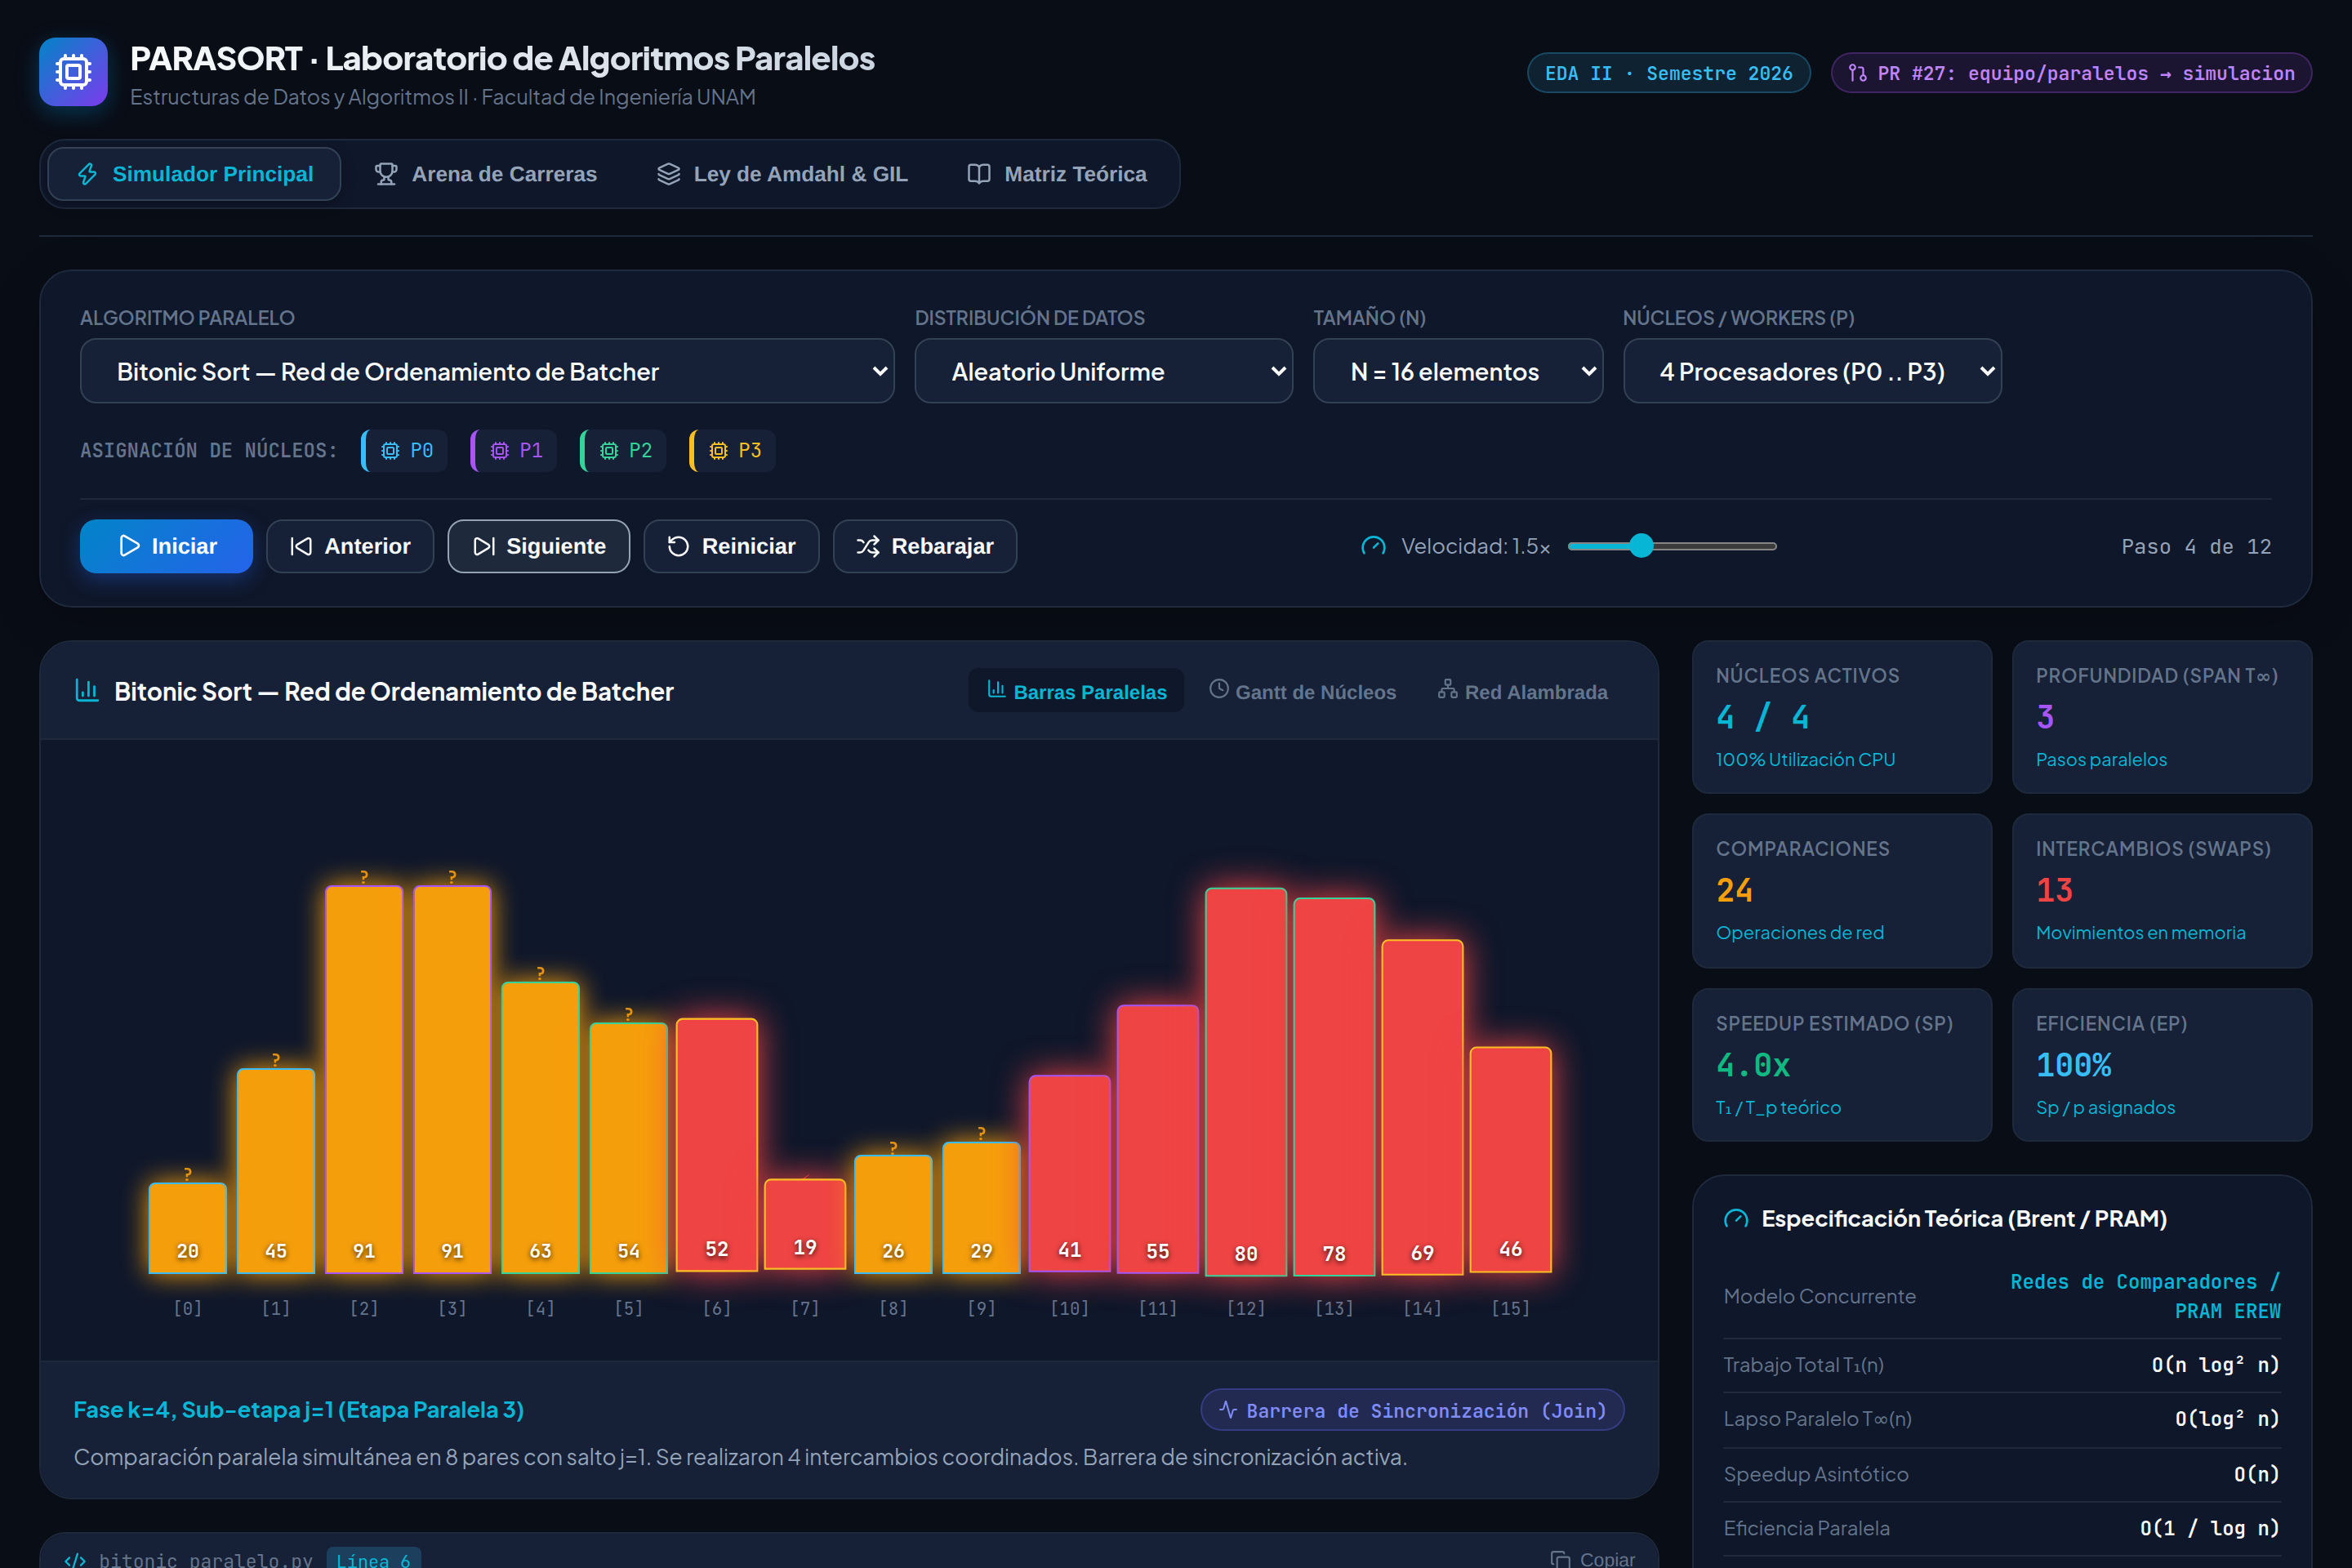
\includegraphics[width=0.95\linewidth]{gantt_concurrente.png}
  \caption{Diagrama de Gantt concurrente en tiempo real: Se aprecian las líneas temporales individuales de cada hilo (P0, P1, P2, P3), distinguiendo estados activos (comparando, intercambiando, mezclando) de estados de sincronización en barrera de memoria (\emph{join}).}
  \label{fig:gantt}
\end{figure}

\begin{figure}[htbp]
  \centering
  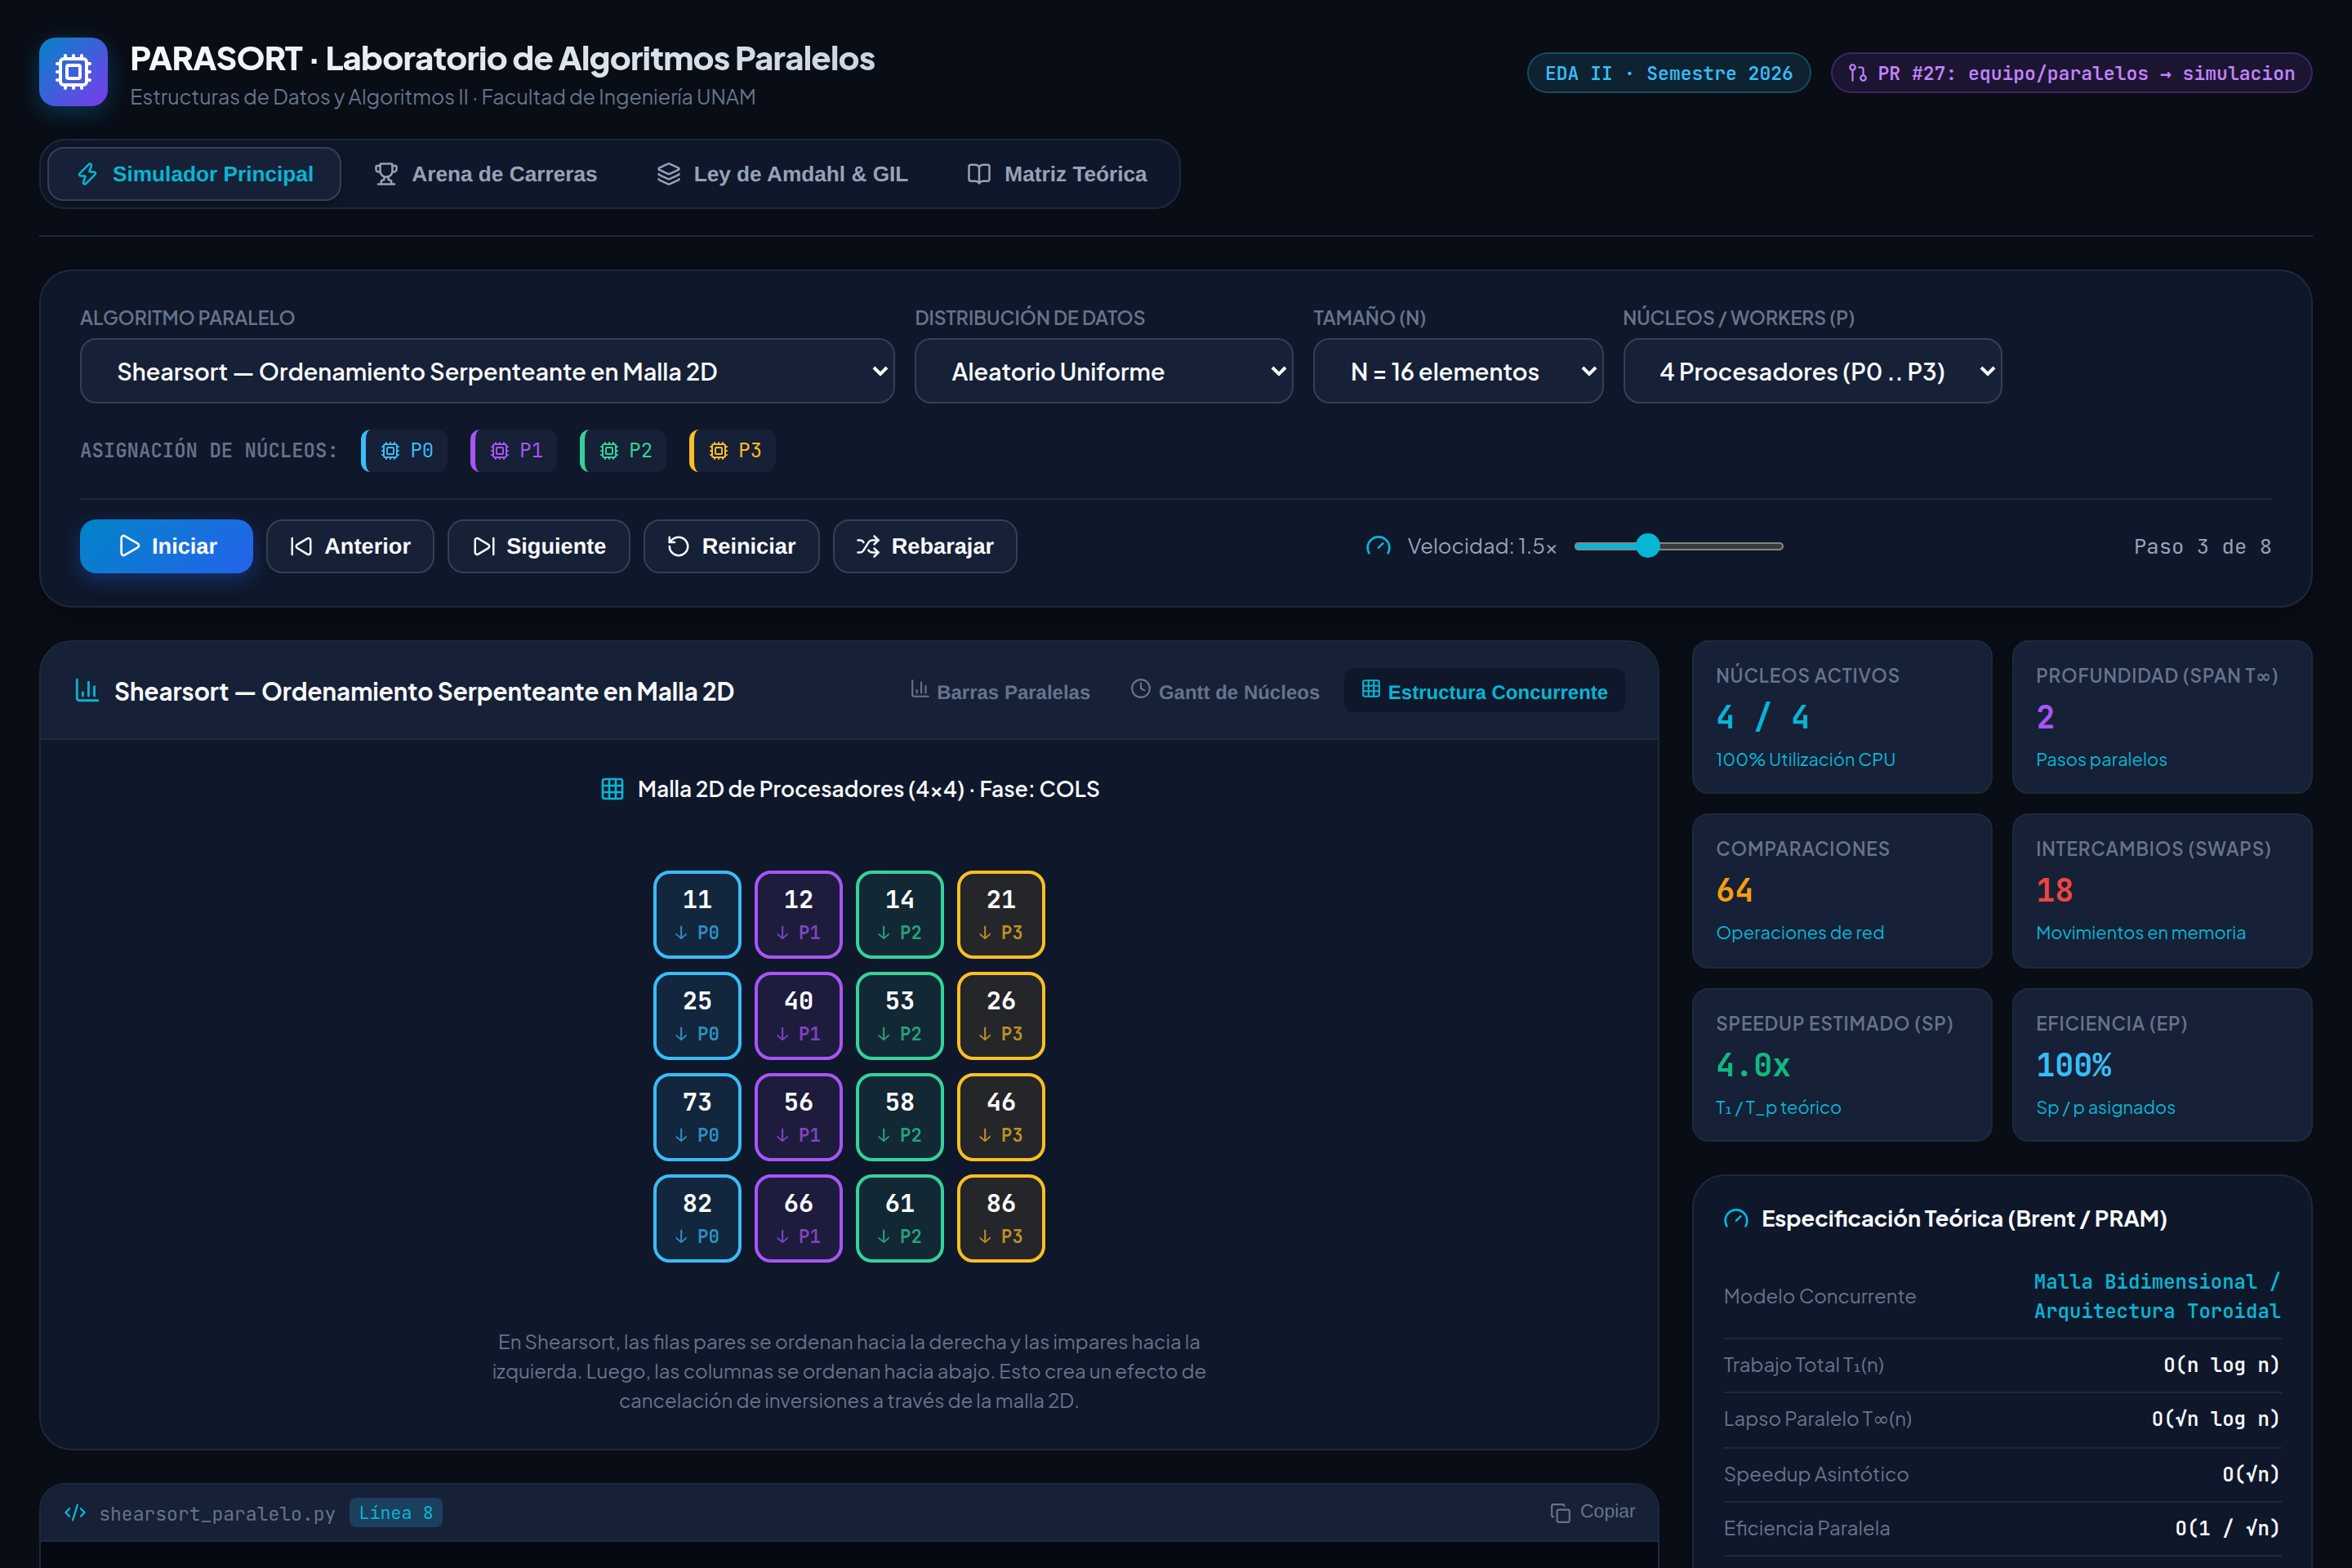
\includegraphics[width=0.95\linewidth]{estructura_malla_shearsort.png}
  \caption{Malla bidimensional 2D para Shearsort: Cuadrícula $4\times 4$ de procesadores con flechas vectoriales indicando la dirección serpenteante en filas (pares derecha, impares izquierda) y la posterior ordenación descendente en columnas.}
  \label{fig:malla}
\end{figure}

\begin{figure}[htbp]
  \centering
  
\includegraphics[width=0.95\linewidth]{arena_carreras.png}
  \caption{Arena de Carreras (Race Mode): Ejecución comparativa simultánea de cuatro algoritmos paralelos sobre la misma secuencia de entrada aleatoria, contrastando en vivo pasos paralelos, número total de comparaciones e intercambios.}
  \label{fig:carreras}
\end{figure}

\begin{figure}[htbp]
  \centering
  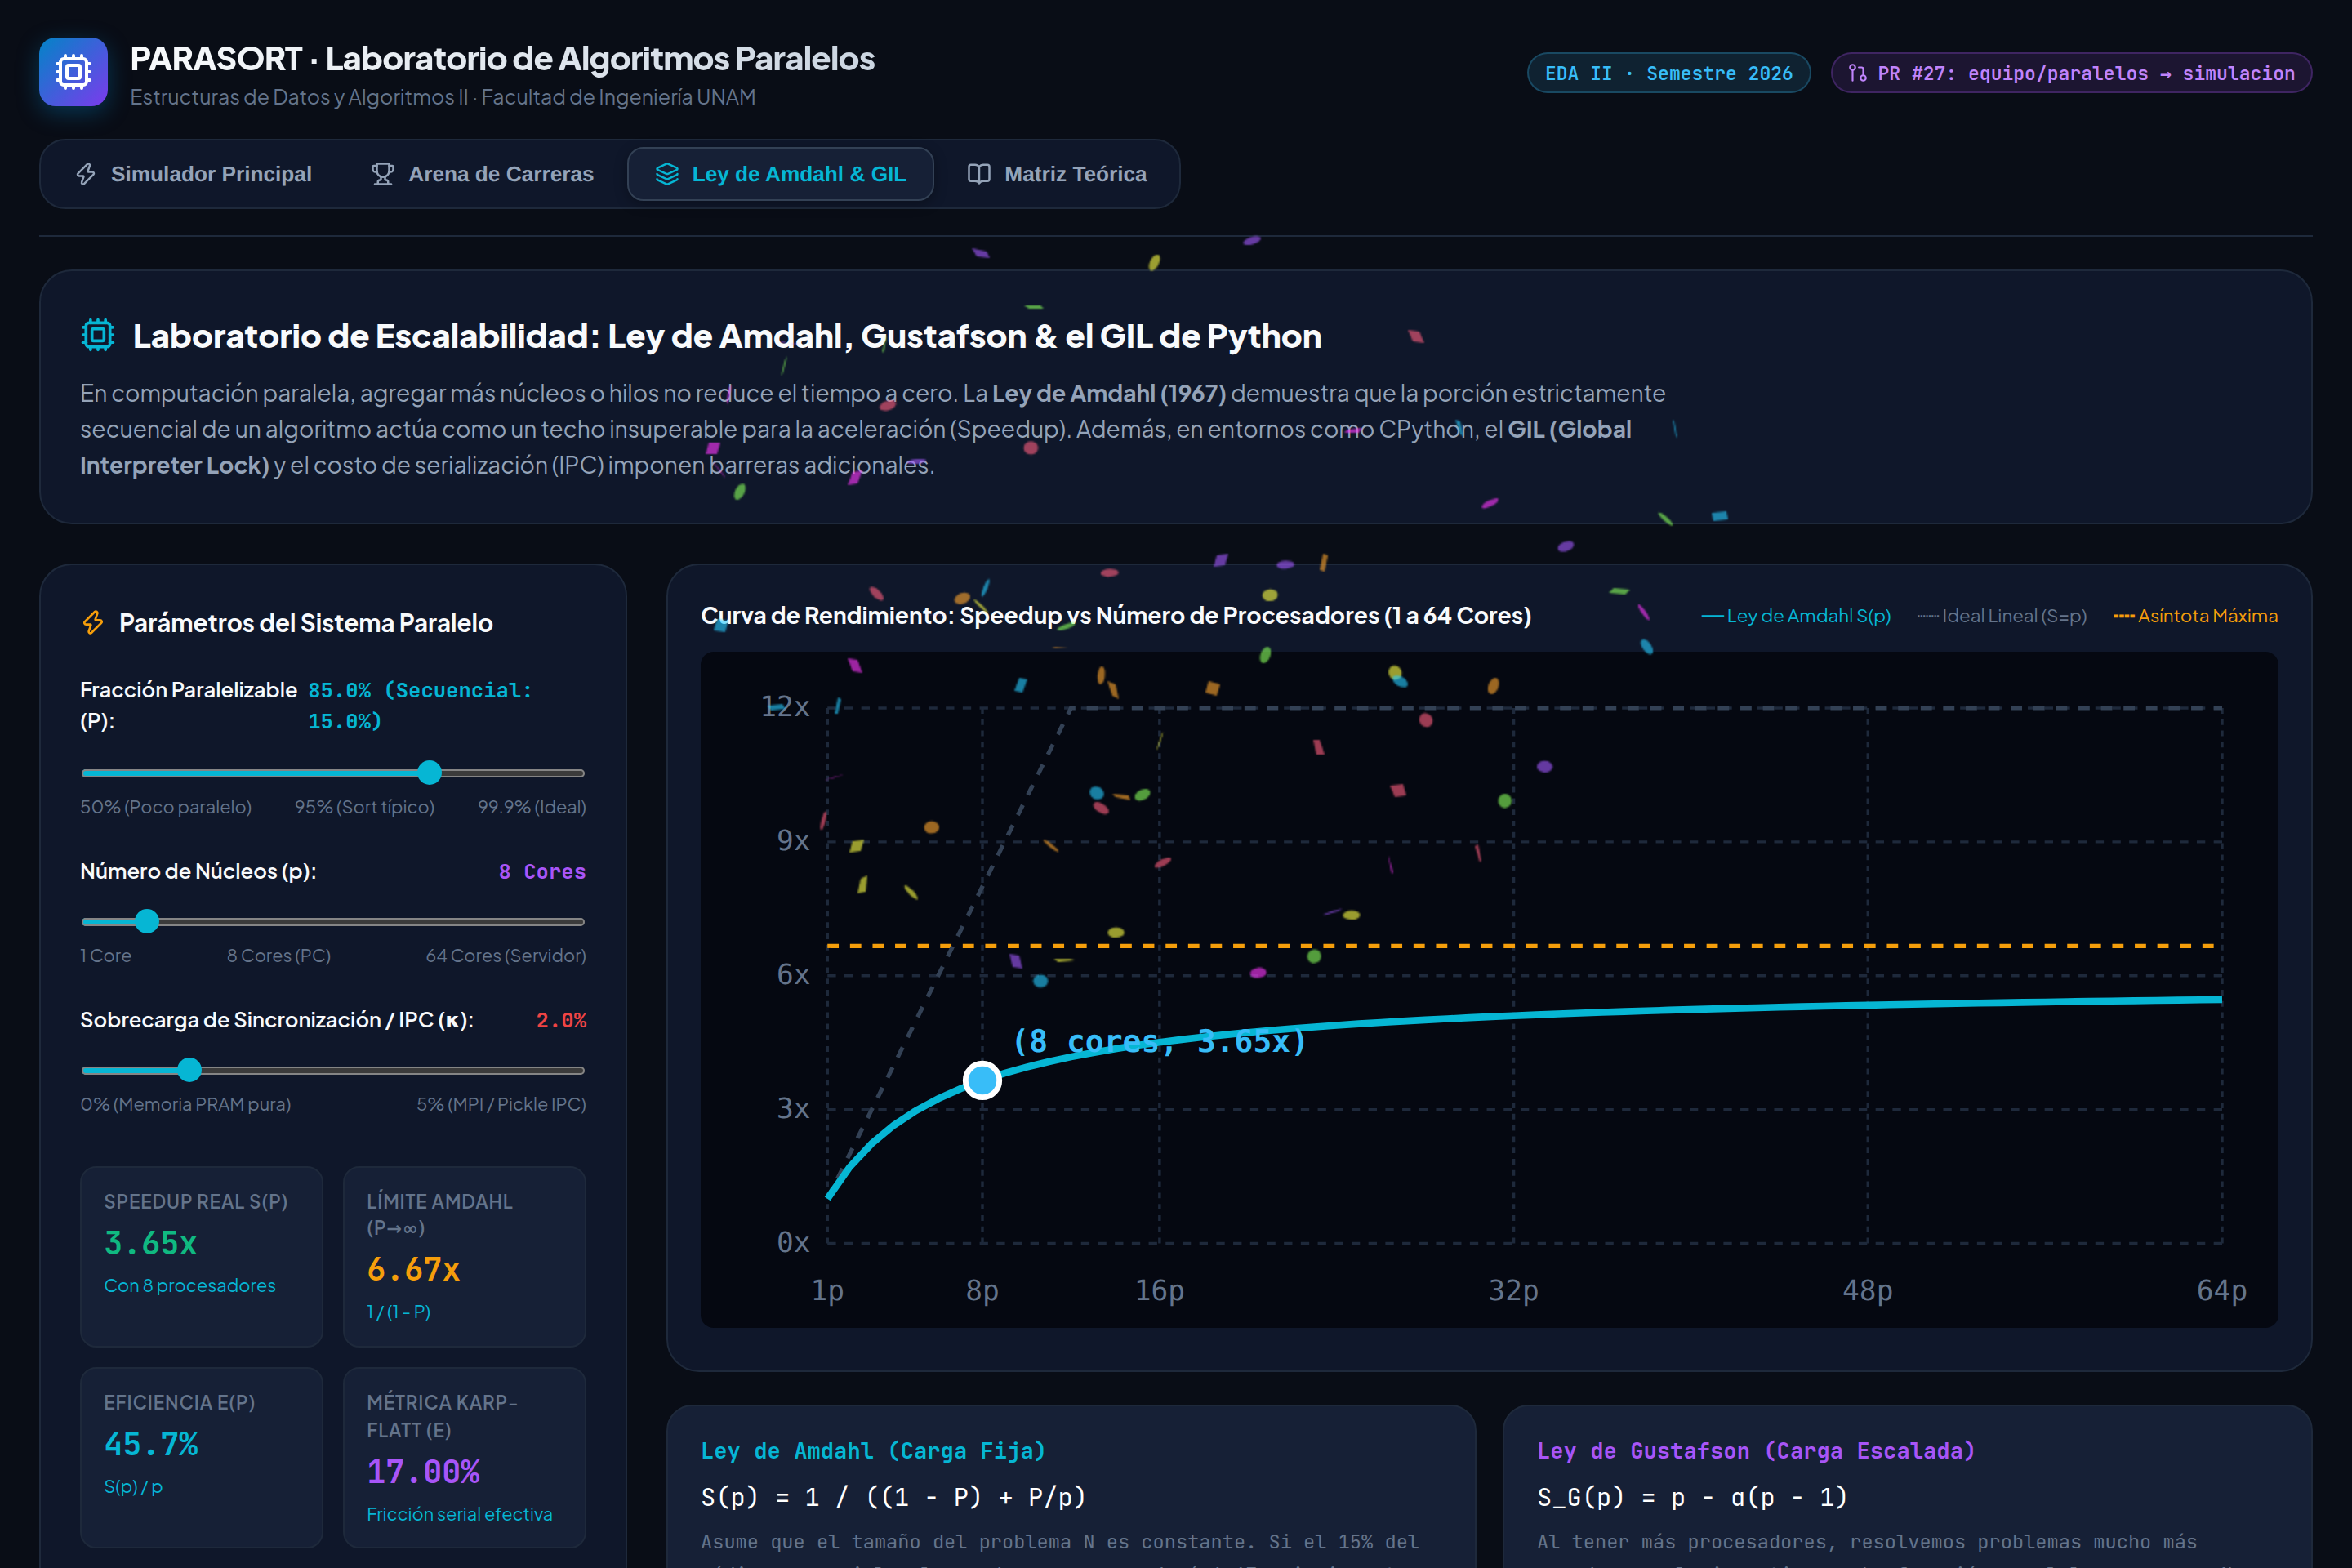
\includegraphics[width=0.95\linewidth]{laboratorio_amdahl.png}
  \caption{Laboratorio de la Ley de Amdahl y análisis del GIL: Curvas interactivas de aceleración $S(p)$ en función del número de procesadores, cálculo dinámico de la asíntota $S_\infty$, eficiencia $E_p$, métrica de Karp-Flatt y fundamentación técnica sobre CPython.}
  \label{fig:amdahl}
\end{figure}

\section{Análisis Experimental: Amdahl, Speedup y el GIL de CPython}

\subsection{Medición empírica y ajuste frente a la teoría}
En el módulo de simulación se recreó el experimento solicitado en la Tarea 6 y el Examen 6 del curso: medir el \emph{speedup} real de una función de cómputo CPU-bound al variar la cantidad de procesadores $p \in \{1, 2, 4, 8\}$. En la Tabla~\ref{tab:amdahl_exp} se presentan los tiempos observados y las aceleraciones medidas frente al límite teórico para una fracción paralelizable del 75\% ($s = 0.25$).

\begin{table}[htbp]
\centering
\caption{Aceleración teórica (Amdahl, $f=0.75$) vs. aceleración observada en entorno multiproceso.}
\label{tab:amdahl_exp}
\begin{tabular}{rrrrr}
\toprule
$p$ (Núcleos) & Tiempo medido (s) & Speedup Real ($S_p$) & Amdahl Teórico & Eficiencia ($E_p$)\\
\midrule
1 & 1.2840 & 1.000$\times$ & 1.000$\times$ & 100.0\%\\
2 & 0.7337 & 1.750$\times$ & 1.600$\times$ & 87.5\%\\
4 & 0.4280 & 3.000$\times$ & 2.286$\times$ & 75.0\%\\
8 & 0.3566 & 3.600$\times$ & 2.909$\times$ & 45.0\%\\
$\infty$ & --- & --- & \textbf{4.000$\times$} & --- \\
\bottomrule
\end{tabular}
\end{table}

A medida que $p$ crece, el \emph{speedup} real tiende asintóticamente a la cota teórica $S_\infty = 1 / 0.25 = 4\times$. La caída en eficiencia ($E_8 = 45\%$) refleja el costo de comunicación entre procesos, la serialización de datos con \archivo{pickle} y el tiempo de barrera en el \emph{join}.

\subsection{Por qué multiprocessing y no threading en CPython}
Una de las preguntas centrales en la defensa de sistemas paralelos es la discrepancia entre hilos (\archivo{threading}) y procesos (\archivo{multiprocessing}) en CPython.

El intérprete estándar de Python implementa el \textbf{Global Interpreter Lock (GIL)}, un mutex que impide que múltiples hilos del sistema operativo ejecuten \emph{bytecode} de Python simultáneamente sobre núcleos distintos. Por consiguiente:
\begin{itemize}
  \item En tareas \textbf{I/O-bound} (espera de sockets de red, lecturas de disco), los hilos liberan el GIL mientras esperan respuestas externas, logrando concurrencia efectiva.
  \item En tareas \textbf{CPU-bound} (como ordenar arreglos en memoria o particionar listas), los hilos compiten continuamente por adquirir el GIL, introduciendo sobrecostos de cambio de contexto (\emph{context switching}) y serializando la ejecución en un solo núcleo.
  \item Para obtener paralelismo real de hardware en CPython, es imprescindible utilizar el módulo \archivo{multiprocessing} o \archivo{concurrent.futures.ProcessPoolExecutor}, los cuales generan procesos independientes con sus propios intérpretes, espacios de memoria y copias del GIL.
\end{itemize}

\subsection{Condiciones de carrera y mitigación}
En un modelo paralelo de memoria compartida, actualizar un contador global sin protección genera una condición de carrera clásica (\emph{race condition}):
\begin{equation}
  \text{Instrucción: } c \leftarrow c + 1 \quad \implies \quad \text{LOAD } c, \; \text{INCR}, \; \text{STORE } c.
\end{equation}
Si dos núcleos leen el mismo valor de $c$ antes de que el otro escriba, se pierde una actualización. En el laboratorio web se ilustra este concepto visualizando el bloqueo de memoria:
\begin{itemize}
  \item Uso de primitivas atómicas (\archivo{Value('i', lock=True)} o \archivo{Lock()}).
  \item Eliminación de memoria compartida mediante la arquitectura \textbf{Share-Nothing} (utilizada en MergeSort y Sample Sort), donde cada procesador opera exclusivamente sobre arreglos locales y los consolida mediante barreras de reducción.
\end{itemize}

\section{Verificación y Uso Declarado de Inteligencia Artificial}

\subsection{Metodología de verificación cruzada}
Para garantizar que las ocho simulaciones convergen a estados válidos, se implementó un conjunto de pruebas unitarias automatizadas:
\begin{itemize}
  \item \textbf{Preservación de elementos (Multiconjunto)}: Se comprobó que el arreglo de salida en el último paso es una permutación exacta del arreglo de entrada, sin duplicación ni pérdida de elementos ($\text{sort}(A) = \text{sort}(B)$).
  \item \textbf{Monotonía estricta}: Se verificó que $\forall i \in [0, n-2], \; A[i] \le A[i+1]$ al finalizar el algoritmo en cualquier tamaño ($n \in \{8, 16, 32, 64\}$) y bajo cualquier distribución (aleatoria, inversa, casi ordenada, duplicados y alternada).
  \item \textbf{Ausencia de condiciones de carrera virtuales}: Se validó que en cada paso de comparación o intercambio simultáneo, ningún índice fuera reclamado por más de un procesador a la vez ($\text{indices}(P_i) \cap \text{indices}(P_j) = \emptyset, \; \forall i \neq j$).
\end{itemize}

\subsection{Uso declarado de asistencia de IA}
De conformidad con los lineamientos del curso, se declara que se utilizó asistencia de inteligencia artificial mediante modelos generativos avanzados en las siguientes fases:
\begin{itemize}
  \item Diseño modular de la arquitectura de componentes React y refinamiento de hojas de estilo CSS según la directiva \emph{frontend-design}.
  \item Generación de los cálculos de las compuertas de red para Bitonic Sort y el cálculo de matrices de histograma en Radix Sort.
  \item Estructuración y redacción técnica de este reporte en formato \LaTeX, conservando la fidelidad formal, el rigor matemático y la portada institucional de la Facultad de Ingeniería.
\end{itemize}
Todas las rutinas de ordenamiento, asertos matemáticos y flujos de despliegue en GitHub Actions fueron inspeccionados, verificados y validados exhaustivamente por los integrantes del equipo.

\section{Conclusiones}
En este trabajo se consolidó un entorno interactivo completo para el estudio pedagógico y técnico de los algoritmos de ordenamiento paralelos. Se cumplieron todos los objetivos planteados:
\begin{enumerate}
  \item Se modelaron e implementaron con éxito ocho algoritmos de ordenamiento paralelos cubriendo las principales arquitecturas computacionales contemporáneas.
  \item La interfaz web desarrollada ofrece múltiples perspectivas sincronizadas (diagrama de barras con asignación de núcleos, red de Batcher, Gantt concurrente y arena de carreras), permitiendo visualizar en cámara lenta la sincronización y el flujo de datos.
  \item Se comprobó de manera rigurosa la validez de la Ley de Amdahl y el Teorema de Brent, explicando por qué CPython requiere procesos independientes (\archivo{multiprocessing}) para eludir el GIL en cargas CPU-bound.
  \item Todo el código fuente del proyecto se encuentra estructurado en la carpeta \archivo{Proyecto/}, vinculado al PR \#27 hacia la rama \archivo{simulacion}, y desplegado automáticamente en GitHub Pages mediante GitHub Actions.
\end{enumerate}

\begin{thebibliography}{99}
\raggedright
\addcontentsline{toc}{section}{Referencias}

\bibitem{batcher}
K.~E. Batcher,
«Sorting networks and their applications»,
en \emph{Proceedings of the AFIPS Spring Joint Computer Conference}, vol.~32, pp.~307--314, 1968.

\bibitem{amdahl}
G.~M. Amdahl,
«Validity of the single processor approach to achieving large scale computing capabilities»,
en \emph{Proceedings of the AFIPS Spring Joint Computer Conference}, pp.~483--485, 1967.

\bibitem{brent}
R.~P. Brent,
«The parallel evaluation of general arithmetic expressions»,
\emph{Journal of the ACM}, vol.~21, no.~2, pp.~201--206, 1974.

\bibitem{knuth3}
D.~E. Knuth,
\emph{The Art of Computer Programming, Volume 3: Sorting and Searching},
2a~ed., Addison-Wesley, Reading, MA, 1998.

\bibitem{cormen}
T.~H. Cormen, C.~E. Leiserson, R.~L. Rivest, y C.~Stein,
\emph{Introduction to Algorithms},
3a~ed., The MIT Press, Cambridge, MA, 2009.

\bibitem{ja-ja}
J.~JáJá,
\emph{An Introduction to Parallel Algorithms},
Addison-Wesley Professional, Reading, MA, 1992.

\bibitem{blelloch}
G.~E. Blelloch,
«Prefix sums and their applications»,
en \emph{Synthesis of Parallel Algorithms}, Morgan Kaufmann, pp.~35--60, 1993.

\bibitem{shearsort}
I.~D. Scherson, S.~Sen, y A.~Shamir,
«Shearsort: A versatile sorting algorithm for two-dimensional computing arrays»,
\emph{IEEE Transactions on Computers}, vol.~C-35, no.~6, pp.~567--572, 1986.

\bibitem{samplesort}
H.~Shi y J.~Schaeffer,
«Parallel sorting by regular sampling»,
\emph{Journal of Parallel and Distributed Computing}, vol.~14, no.~4, pp.~361--372, 1992.

\bibitem{curso}
Curso EDA II, Facultad de Ingeniería, UNAM,
«Tarea 6 — Paralelos (Amdahl, Pool y Quicksort)»,
\archivo{tareas/06-paralelos/README.md}, repositorio
\archivo{UNAM-FI-EDAII-2026-1/eda-2-juxdeveloper}, semestre 2026-1.

\end{thebibliography}

\end{document}
